\documentclass[conference]{IEEEtran}
% \IEEEoverridecommandlockouts
% The preceding line is only needed to identify funding in the first footnote. If that is unneeded, please comment it out.
\usepackage{amsmath,amssymb,amsfonts}
\usepackage{algorithmic}
\usepackage{graphicx}
\usepackage{textcomp}
\usepackage{xcolor}
\usepackage{hyperref}
\usepackage{csquotes}
\usepackage{tikz}
\usetikzlibrary{arrows.meta, positioning, shapes.geometric, fit}
\usepackage[backend=biber,style=ieee]{biblatex}
\addbibresource{references.bib}
\def\BibTeX{{\rm B\kern-.05em{\sc i\kern-.025em b}\kern-.08em
    T\kern-.1667em\lower.7ex\hbox{E}\kern-.125emX}}
\begin{document}

\title{
Multimodal Seizure Prediction Using EEG Time-Series Features and Clinical Metadata
% TODO: Edit GitHub repo and documentation to use a more descriptive name (TBD)
\thanks{Code available at: \url{https://github.com/lukeblevins/eeg-Spr2026-CSCI7090}}
}

\author{
\IEEEauthorblockN{Luke Blevins}
\IEEEauthorblockA{Department of Computer Science\\
Georgia Southern University\\
Statesboro, United States \\
lb22835@georgiasouthern.edu}
\and
\IEEEauthorblockN{Jacob Rawlins}
\IEEEauthorblockA{Department of Computer Science\\
Georgia Southern University\\
Statesboro, United States \\
jr29003@georgiasouthern.edu}
\and
\IEEEauthorblockN{Arnoldo Vilches-Arteaga}
\IEEEauthorblockA{Department of Computer Science\\
Georgia Southern University\\
Statesboro, United States \\
av05604@georgiasouthern.edu}
}

\maketitle


\begin{abstract}
Millions of people worldwide suffer from a neurological condition known as epilepsy, which causes recurring seizures in those afflicted. These seizures and their symptoms vary widely from person to person, making diagnosis and treatment difficult for medical professionals. Electroencephalography (EEG) recordings are used not only to diagnose but to predict epileptic seizures. Machine learning algorithms using these recordings have emerged over the years as a useful tool for epileptic seizure prediction. This systematic literature review aims to analyze the accuracy and performance of these models. A review of recent research on this topic was conducted, resulting in the inclusion of 12 articles. The reviewed studies show a lack of standardization in epileptic seizure prediction, making comparisons and analyses of models difficult. While machine learning shows potential for seizure prediction, challenges still remain that limit its use in clinical settings. Code available at: \url{https://github.com/lukeblevins/eeg-Spr2026-CSCI7090}
\end{abstract}

\begin{IEEEkeywords}
Electroencephalography, epilepsy, deep learning, machine learning
\end{IEEEkeywords}

\section{Introduction}
Epilepsy is considered one of the most common neurological disorders, affecting an estimated 50 million people worldwide \cite{who2024epilepsy}. It causes recurring seizures in those afflicted, which involve moments of involuntary movement and, in some cases, the loss of consciousness \cite{who2024epilepsy}. Although people with epilepsy can live normal lives, they still face serious risks such as an increased chance of disability or even death \cite{ninds2025epilepsy}. Therefore, the use of machine learning models for seizure prediction would significantly improve patients' quality of life by giving them time to prepare and seek medical attention. 

There are many methods for properly diagnosing epileptic seizures, such as the electroencephalogram (EEG), which measures electrical activity in the brain and identifies abnormalities \cite{ninds2025epilepsy}. EEG data is also used by machine learning models to predict epileptic seizures by detecting the preictal state, which is the time period preceding a seizure \cite{mourad2025seizurerecognition}. There is extensive research on machine learning approaches for epileptic seizure prediction; however, current research lacks standardization, making the analysis of existing models difficult. This systematic review aims to analyze these models through the following research questions:

\begin{itemize}
\item \textbf{RQ1:} What EEG features matter most, and how should they be extracted?

\item \textbf{RQ2:} How and where should metadata be fused into the model?

\item \textbf{RQ3:} What architecture best handles the multimodal, temporal nature of the data?

\item \textbf{RQ4:} Can the model work across patients?

\end{itemize}

\section{Methodology}
For this systematic literature review, the scientific databases searched were PubMed, IEEE Xplore, and ScienceDirect. The keywords used in the search included “EEG”, “seizure prediction”, “epilepsy”, “deep learning”, “neural networks”, and “machine learning”. The resulting articles were reviewed by title and abstract to ensure relevance to the topic, and then screened against the inclusion and exclusion criteria.  

\subsection{Inclusion Criteria}
\begin{itemize}
  \item \textbf{1:} Articles published between 2021 and the present date.
  \item \textbf{2:} Articles written in English.
  \item \textbf{3:} Peer-reviewed articles published in a reputable journal.
  \item \textbf{4:} Articles that have been cited in numerous other articles.
\end{itemize}

\subsection{Exclusion Criteria}
\begin{itemize}
  \item \textbf{1:} Articles on animal studies rather than human.
  \item \textbf{2:} Articles that did not use seizure or EEG data.
  \item \textbf{3:} Articles foucssed primarily on seizure dection opposed to prediction.
  \item \textbf{4:} Articles that are not peer-reviewed.
\end{itemize}

% Add to preamble if not already present:
% \usepackage{tikz}
% \usetikzlibrary{arrows.meta, positioning, shapes.geometric, fit}

\begin{figure*}[t]
\centering
\resizebox{\textwidth}{!}{
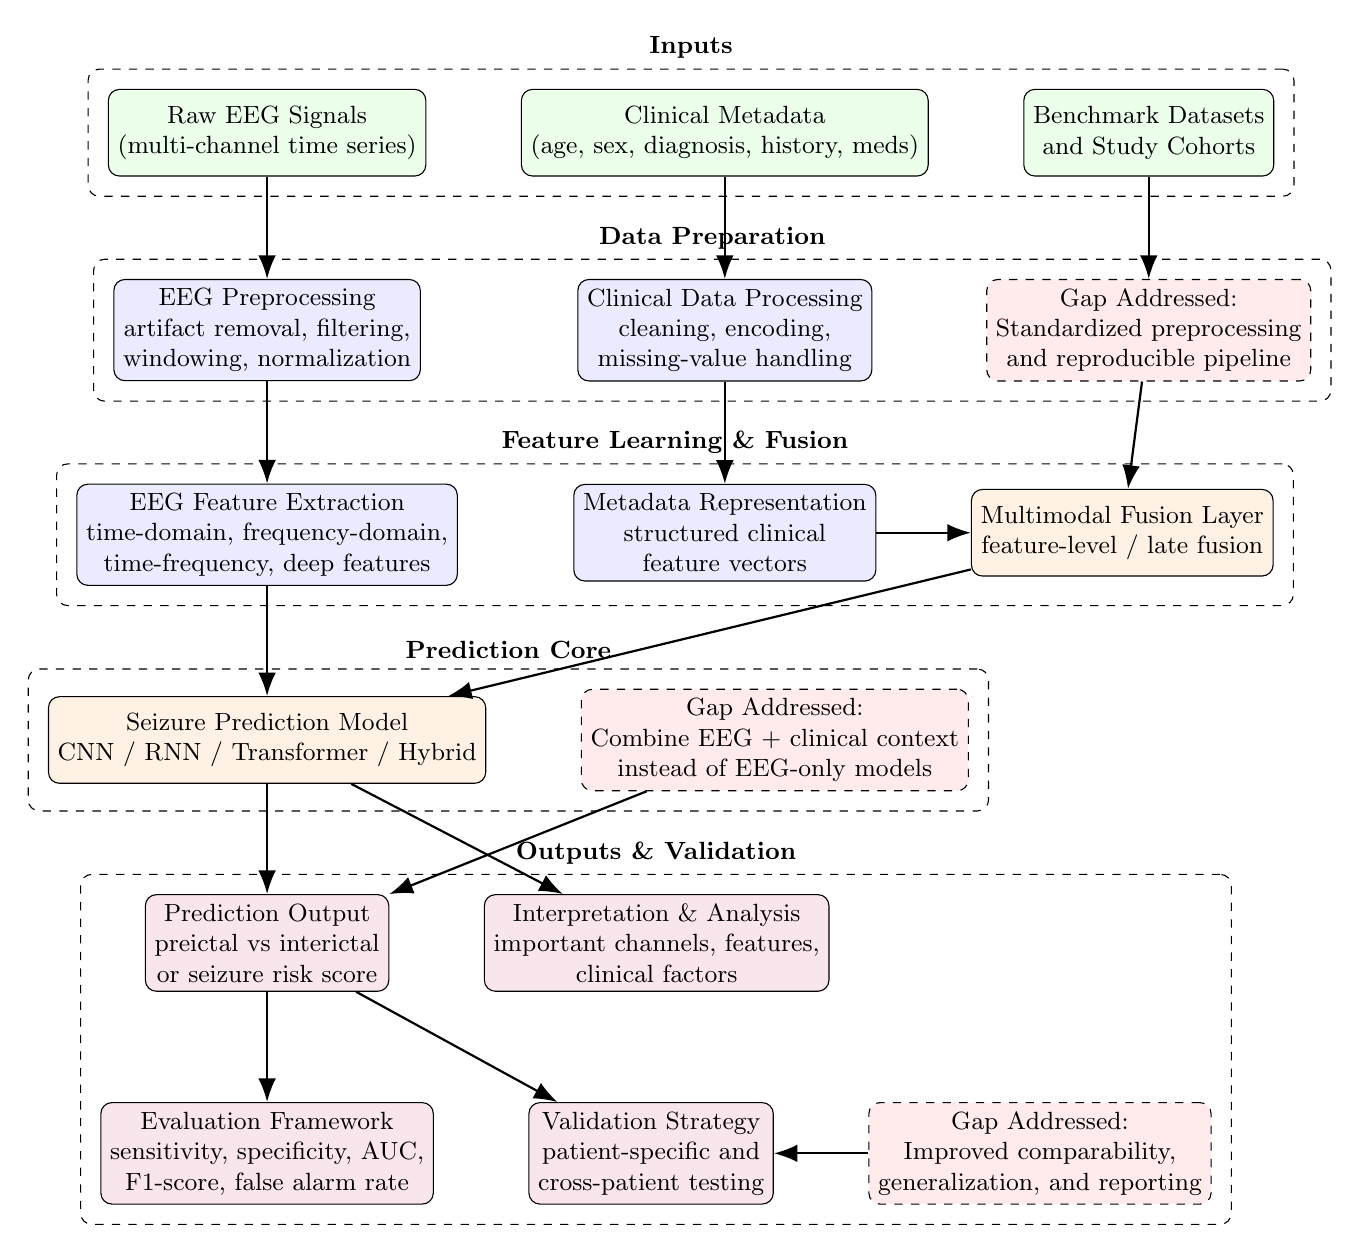
\begin{tikzpicture}[
    font=\small,
    node distance=0.9cm and 1.2cm,
    >=Latex,
    box/.style={
        draw,
        rounded corners,
        align=center,
        minimum width=3.0cm,
        minimum height=1.1cm
    },
    process/.style={
        box,
        fill=blue!8
    },
    data/.style={
        box,
        fill=green!8
    },
    model/.style={
        box,
        fill=orange!10
    },
    eval/.style={
        box,
        fill=purple!10
    },
    gap/.style={
        box,
        fill=red!8,
        dashed
    },
    line/.style={
        -{Latex[length=3mm]},
        thick
    }
]

% Row 1: Inputs
\node[data] (eeg) {Raw EEG Signals\\(multi-channel time series)};
\node[data, right=of eeg] (clinical) {Clinical Metadata\\(age, sex, diagnosis, history, meds)};
\node[data, right=of clinical] (datasets) {Benchmark Datasets\\and Study Cohorts};

% Row 2: Preprocessing
\node[process, below=1.3cm of eeg] (preprocess) {EEG Preprocessing\\artifact removal, filtering,\\windowing, normalization};
\node[process, below=1.3cm of clinical] (clinprep) {Clinical Data Processing\\cleaning, encoding,\\missing-value handling};
\node[gap, below=1.3cm of datasets] (gap1) {Gap Addressed:\\Standardized preprocessing\\and reproducible pipeline};

% Row 3: Features
\node[process, below=1.3cm of preprocess] (eegfeat) {EEG Feature Extraction\\time-domain, frequency-domain,\\time-frequency, deep features};
\node[process, below=1.3cm of clinprep] (clinfeat) {Metadata Representation\\structured clinical\\feature vectors};
\node[model, right=1.2cm of clinfeat] (fusion) {Multimodal Fusion Layer\\feature-level / late fusion};

% Row 4: Model
\node[model, below=1.4cm of eegfeat] (predictor) {Seizure Prediction Model\\CNN / RNN / Transformer / Hybrid};
\node[gap, right=1.2cm of predictor] (gap2) {Gap Addressed:\\Combine EEG + clinical context\\instead of EEG-only models};

% Row 5: Outputs
\node[eval, below=1.4cm of predictor] (output) {Prediction Output\\preictal vs interictal\\or seizure risk score};
\node[eval, right=of output] (explain) {Interpretation \& Analysis\\important channels, features,\\clinical factors};

% Row 6: Evaluation
\node[eval, below=1.4cm of output] (evaluation) {Evaluation Framework\\sensitivity, specificity, AUC,\\F1-score, false alarm rate};
\node[eval, right=of evaluation] (generalization) {Validation Strategy\\patient-specific and\\cross-patient testing};
\node[gap, right=of generalization] (gap3) {Gap Addressed:\\Improved comparability,\\generalization, and reporting};

% Arrows
\draw[line] (eeg) -- (preprocess);
\draw[line] (clinical) -- (clinprep);
\draw[line] (datasets) -- (gap1);

\draw[line] (preprocess) -- (eegfeat);
\draw[line] (clinprep) -- (clinfeat);

\draw[line] (eegfeat) -- (predictor);
\draw[line] (clinfeat) -- (fusion);
\draw[line] (fusion) -- (predictor);

\draw[line] (predictor) -- (output);
\draw[line] (predictor) -- (explain);
\draw[line] (output) -- (evaluation);
\draw[line] (output) -- (generalization);

\draw[line] (gap1) -- (fusion);
\draw[line] (gap2) -- (output);
\draw[line] (gap3) -- (generalization);

% Optional grouping boxes
\node[draw, dashed, rounded corners, inner sep=0.25cm, fit=(eeg)(clinical)(datasets), label=above:{\textbf{Inputs}}] {};
\node[draw, dashed, rounded corners, inner sep=0.25cm, fit=(preprocess)(clinprep)(gap1), label=above:{\textbf{Data Preparation}}] {};
\node[draw, dashed, rounded corners, inner sep=0.25cm, fit=(eegfeat)(clinfeat)(fusion), label=above:{\textbf{Feature Learning \& Fusion}}] {};
\node[draw, dashed, rounded corners, inner sep=0.25cm, fit=(predictor)(gap2), label=above:{\textbf{Prediction Core}}] {};
\node[draw, dashed, rounded corners, inner sep=0.25cm, fit=(output)(explain)(evaluation)(generalization)(gap3), label=above:{\textbf{Outputs \& Validation}}] {};

\end{tikzpicture}
}
\caption{Overview of the proposed multimodal seizure prediction pipeline integrating EEG signals and clinical metadata, with explicit design choices to address key literature gaps in preprocessing standardization, multimodal fusion, and generalizable evaluation.}
\label{fig:framework}
\end{figure*}

\section{Literature Review}
Accurate epileptic seizure diagnosis remains clinically challenging because seizure events are often unwitnessed or incompletely described. In addition, specialized expertise for analyzing EEG data is limited, and patients may therefore present to non-experts for initial evaluation.

Recent systematic reviews and methodological surveys indicate a growing body of work applying machine learning and deep learning to EEG-based seizure prediction and related epilepsy assessment tasks \cite{han2024epilepsycare,li2025signalsanalysis,vallabhaneni2021eegdecoding}. Han \textit{et al.} \cite{han2024epilepsycare} review AI/ML applications for epilepsy and seizure diagnosis across modalities (including EEG, neuroimaging, wearables, and seizure video) and emphasize that clinical integration depends on generalizability, interpretability, and consistent reporting practices. Complementing this perspective, Li \textit{et al.} \cite{li2025signalsanalysis} provide a methodological synthesis of deep learning for EEG and intracranial EEG (iEEG) analysis and formalize evaluation strategies (subject-specific, mixed-subject, and cross-subject), arguing that cross-subject testing best reflects deployment on previously unseen patients. Vallabhaneni \textit{et al.} \cite{vallabhaneni2021eegdecoding} survey deep learning approaches for EEG decoding and note persistent practical constraints, including hyperparameter sensitivity, computational cost, and limited robustness across subjects and acquisition settings. These themes motivate careful validation design and transparent performance reporting in seizure prediction research.

Multiple studies have shifted towards the use of deep learning architectures designed to identify discriminative features during the preictal phase, the period preceding seizure onset. This literature review analyzes recent systematic reviews as well as experimental studies to identify current methodological practices in the field, highlight gaps and weaknesses, and discuss emerging trends \cite{carmo2024seizureforecast,shafiezadeh2024crosspatient,mourad2025seizurerecognition,sobhona2023sysreview}.

Synthesizing the reviewed evidence, a central methodological direction is to integrate seizure forecasting signals directly into seizure prediction pipelines rather than treating prediction as a standalone binary classification task. Forecast-oriented features such as time-varying preictal risk scores, individualized warning horizons, and uncertainty estimates can translate EEG-derived patterns into outputs that are more actionable for clinical decision-making. This integrated framing links model accuracy to real-world utility and sets the stage for forecast-focused evaluation strategies in the studies discussed next \cite{carmo2024seizureforecast}. % add more studies here that support this

Aligned with this synthesis, Carmo \textit{et al.} in ``Automated algorithms for seizure forecast: a systematic review and meta-analysis'' \cite{carmo2024seizureforecast} provide a foundational effort to formalize forecast-oriented seizure modeling. This article provides a systematic review of patient-specific seizure forecasting algorithms to assess reported performance and establish reference points for future developments. The authors discuss the lack of standardization in seizure forecasting research and unclear performance benchmarks, and note the need to distinguish between forecasting and prediction while improving evaluation practices. To investigate these issues, the authors followed PRISMA guidelines, resulting in the analysis of 18 studies containing 43 seizure forecast algorithms. The results show high variability in approaches used across studies. In response, the authors propose guidelines to standardize seizure forecasting and also set benchmarks for future research. The review also emphasizes the need for a clearer distinction between seizure forecasting and prediction. Additionally, the review reports inconsistent use of probabilistic performance metrics and inconsistent definitions of forecast horizons.

While the previous review highlights the need for standardized metrics, another key issue is the heavy reliance on patient-specific data, which is prone to data leakage and overpromising of results. To address this issue, the study titled “A systematic review of cross-patient approaches for EEG epileptic seizure prediction” \cite{shafiezadeh2024crosspatient} examines patient-independent testing to promote more rigorous model assessment practices. The authors followed PRISMA guidelines and selected 21 articles on cross-patient testing by applying inclusion and exclusion criteria. Through this analysis, the authors concluded that relatively few studies use cross-patient testing, with their 21 articles accounting for only 4 percent of the literature. The studies analyzed used cross-patient testing either with or without adaptation. The authors found that seizure prediction remains challenging and that future work should focus on explainable AI models and a standardized workflow for validating prediction models.

In addition to these concerns, questions regarding the effectiveness of models remain. The article “Machine and deep learning methods for epileptic seizure recognition using EEG data: A systematic review” \cite{mourad2025seizurerecognition} evaluates machine and deep learning models for epileptic seizure recognition, which includes detection, prediction, and classification. The authors followed PRISMA guidelines, searched the PubMed database, and applied a screening process that included inclusion and exclusion criteria, resulting in 153 articles analyzed. The review found several challenges in seizure recognition. These include a gap between AI methods and real clinical use, the need for AI models that are easier to interpret, and the lack of clear standards for defining the preictal state. Additionally, the authors found that SVM, CNN, and LSTM were the most effective models for classification, feature extraction, and seizure prediction, respectively \cite{mourad2025seizurerecognition}. However, challenges still prevent the use of recognition models in clinical settings.

Likewise, Jahan et al. in “AI-Based Epileptic Seizure Detection and Prediction in Internet of Healthcare Things: A Systematic Review” reviewed existing research on epileptic seizure recognition using EEG data. The study analyzes published machine learning and deep learning models used for seizure detection and prediction, and evaluates the performance of different classification algorithms. The authors conducted a PRISMA-guided process for their article selection, resulting in the inclusion of 56 studies. In their systematic review, the authors found that SVM, RF, and KNN are the most powerful machine learning classifiers \cite{sobhona2023sysreview}. These classifiers are commonly applied in seizure prediction models. The review also highlights current challenges, such as the lack of publicly available long-term EEG datasets, heterogeneity between seizures, and the black-box nature of machine learning. The authors also suggest that future works should focus on explainable AI, multimodal classification algorithms, and the use of wireless EEG headsets to aid in the long term EEG data collection \cite{sobhona2023sysreview}.

Building upon the previous article, the study titled ``Neural networks for epilepsy detection and prediction with EEG signals: a systematic review'' provides a large scoping analysis of neural-network-based approaches in EEG seizure research. This study provides a broader overview, including seizure prediction as well as seizure detection. Using the PRISMA methodology, 341 studies were selected through inclusion and exclusion criteria. The review analyzes datasets, preprocessing, architectures, and results to identify common pipeline components as well as recurring limitations. Similar to prior reviews, this study highlights reliance on limited datasets, frequent use of patient-specific modeling, and inconsistent evaluation metrics.

Extending the findings of previous systematic reviews, the study ``A Review of Machine Learning and Deep Learning Trends in EEG-Based Epileptic Seizure Prediction'' provides a focused review of EEG-based seizure prediction with an analysis of 149 recent studies. While the previous study emphasizes neural-network approaches broadly, this study analyzes trends across both machine learning and deep learning studies. It reviews dataset usage, preprocessing strategies, validation schemes, and evaluation metrics within seizure prediction pipelines. Consistent with earlier reviews, the authors identify overreliance on limited datasets, inconsistencies in evaluation metrics, and the popularity of convolutional neural network models. The study also notes that repeatedly reported high accuracy may not reflect clinically relevant performance when models are trained and tested under patient-specific or static-dataset conditions.

While systematic reviews provide insight into recurring limitations in seizure prediction research, experimental studies continue to develop new approaches to predict seizures. One example is the study ``Predicting epileptic seizures based on EEG signals using spatial depth features of a 3D-2D hybrid CNN.'' This work proposes a hybrid 3D--2D convolutional neural network to capture spatial and inter-channel relationships in multi-channel EEG data. The model combines 3D and 2D convolutional layers to capture spatial structure and inter-channel correlations without substantially increasing computational complexity. However, limitations described in the systematic reviews remain relevant, as the study is evaluated on static datasets rather than continuous real-time settings and uses patient-specific modeling. As the field advances, stronger evidence for clinical translation will require evaluation on more generalizable data and validation protocols aligned with deployment conditions.
r
\section{Results}
\noindent This review synthesizes recent work on EEG-based seizure prediction. The surveyed papers use different datasets, preprocessing choices, model architectures, and evaluation protocols, which makes direct comparison difficult.

\section{Discussion}
\noindent Across the reviewed literature, commonly noted issues include inconsistent evaluation procedures and inconsistent reporting of metrics. Future studies may improve comparability by addressing this.

\section{Synthesis/ Conclusion}
\noindent The literature on seizure prediction has increasingly focused on the use of deep learning to make meaningful predictions. Many recent studies have utilized hybrid or fusion networks as well as multidimensional transformer architectures to improve model prediction accuracy. Despite these strong advances, many challenges remain in the field. Mutiple reviewed systematic reviews highlight the overreliance on small, static datasets to train models which limits performance inreal life environments. Another significant gap is an overreliance on patient specific data found in commonly used datasets limiting the ability to make strong predictions in a general environment. Additionally, there are not standard agreed upon metrics to properly evaluate model performance across different studies. This project aims to address these gaps by investigating model performance using real time data as well as static data to compare performance under different conditions. In addition, this research aims to propose a more consistent set of evaluation metrics that can be used for stronger comparison among different studies. By addressing these mentioned issues, this study aims to contribute to the development of more accurate and generalizable seizure prediction models which are better fitted for real-world applications.
\nocite{*}
\section{Datasets}
\noindent This study will utilize both real-time as well as static datasets to evaluate performance of models for both data forms. Static datasets are more commonly used in seizure prediction as these datasets provide standarized and cleaned data for training and evaluation. However, real-time data better simulates data that would be passed into a model during real time environments. Real-Time data will be collected BrainFlow which obtains EEG data from connected devices through an API. In addition, two widely used open-source datasets will be used, the CHB-MIT Scalp EEG dataset as well as the Temple University Hospital EEG datset. These datasets provide a diverse collection of EEG data for models to train and make predictions on more general data.
\printbibliography


\end{document}
